\documentclass[conference]{IEEEtran}
\IEEEoverridecommandlockouts
\usepackage[utf8]{inputenc}
\usepackage[T1]{fontenc}
\usepackage{mathptmx}
\usepackage{cite}
\usepackage{amsmath}
\usepackage{graphicx}
\usepackage{textcomp}
\usepackage{xcolor}
\usepackage{booktabs}
\usepackage{url}
\newcommand{\pend}[1]{\textcolor{red}{[#1]}}
\setlength{\textfloatsep}{8pt plus 2pt minus 2pt}
\setlength{\intextsep}{8pt plus 2pt minus 2pt}

\begin{document}

\title{Gains on Synthetic Occlusion Are Not Enough:\\Occlusion Augmentation and Real Occlusion in Person Detection}

\author{\IEEEauthorblockN{Celia Patricia Apaza Hilasaca, Brayan Raul Condori Quispe, Jhan Logan Ramos Quispe}
\IEEEauthorblockA{Universidad Peruana Uni\'on (UPeU), Juliaca, Peru}}

\maketitle

\begin{abstract}
Synthetic occlusion augmentation is used to make person detectors robust to partial visibility, yet its benefit is usually measured on the same artificial occlusion. We ask whether a gain on synthetic occlusion is enough to expect a gain on real, human-annotated occlusion in other datasets. We compare a baseline and an augmented model, with the same data and hyperparameters, in 18 blocks that vary the occluder (patches, silhouettes, diffusion, real geometry and depth order), the detector (YOLOv11 at two sizes, YOLO26s, RT-DETR-l, RetinaNet and Faster R-CNN) and the training domain (117 runs, fine-tuned from COCO). Each block is measured on its synthetic control (17 of 18) and on three real-occlusion sources, by day and by night; hypotheses and rules were fixed before training each block, in an internal registry of an adaptive programme. A cell passes if AP@0.5 improves by at least 2 points with a 95\,\% interval that excludes zero. All 17 controls pass (+2.6 to +60.9). In the primary count, with equal training exposure (33 real cells), 5 pass, 15 rule out +2 points and 13 are inconclusive; the mean gain is +0.96 [+0.34; +1.56] on CityPersons, +0.01 on NightOwls and $-0.94$ on ExDark. Only Faster R-CNN with silhouettes meets the rule on two sources; in post hoc analyses, its gain is not clearly larger for occluded people, it is fragile to between-seed variance, on CityPersons it drops to +0.7 when the visible box is scored, and with MR$^{-2}$ it improves by less than 2 points. Passing a synthetic control is not enough to claim robustness to real occlusion.
\end{abstract}

\begin{IEEEkeywords}
person detection, occlusion, data augmentation, robustness, low light, pre-specified hypotheses
\end{IEEEkeywords}

\section{Introduction}
Person detection with RGB cameras supports surveillance and mobile robotics. Occlusion, a major cause of pedestrian-detection failures~\cite{Dollar2012}, and low light~\cite{Loh2019} tend to coincide at night. In our data, a YOLOv11s fine-tuned on ExDark drops from 0.82 AP@0.5 on unoccluded people to 0.24 on people severely occluded by other people.

A widespread remedy is \emph{synthetic occlusion augmentation}: during training, parts of the person are erased or covered~\cite{Zhong2020,Shang2018synthocc,Chi2020pedhunter}. Its benefit is usually measured on the same artificial occlusion or, when real occlusion is used, within the training dataset (CityPersons, CrowdHuman~\cite{Shao2018crowdhuman}); rarely on genuinely occluded people in other datasets. If the synthetic gain does not carry over, synthetic benchmarks overstate robustness.

\textbf{Gap.} In the literature reviewed (Section~II) we found no study that (i) measures the effect on annotated real occlusion with a synthetic control confirming that the augmentation was learned, (ii) with several real sources, (iii) tests alternative explanations (occluder, detector, domain, data volume, exposure) with controlled experiments and (iv) fixes hypotheses and rules before seeing the results.

\textbf{Objectives and contribution.} The objectives are to measure the degradation caused by occlusion (OE1), the effect of augmentation on synthetic and real occlusion by occluder (OE2), detector (OE3), and domain and data (OE4), and its mechanism (OE5)\footnote{The mapping between objectives, method, evidence and pending work, the literature search and all material cited as ``supplement'' are in the supplementary material.}. We contribute (1) controlled evidence in 18 blocks with five kinds of occluder and six detectors (one-stage, two-stage and transformer); (2) a primary count with intervals, split by training exposure, with specificity (occluded versus visible) and box-convention analyses, showing that passing the synthetic control is not enough; and (3) a reusable minimum protocol: a positive control with unseen occluders; V1 and V3 on the same machine and software version; fixed epochs; at least 5 seeds, with CIs that include their variance; real sources from the same and from other domains; specificity; and a rule fixed in advance. It costs 0.5--2.6 GPU hours per block.

\section{Related work and explanatory framework}
\textbf{Detection under occlusion and low light.} Pedestrian detectors tackle occlusion through architecture and evaluate within one benchmark: by parts or with visible boxes~\cite{Zhang2018orcnn,Zhou2018bibox}, refining anchors from visible parts on CityPersons, Caltech and ECP-night~\cite{Song2022prnet}, or fusing levels with Random Erasing~\cite{Huan2023mlffcsp}. For night driving, a YOLOX with domain transfer raises mAP by 5.9 points without stratifying by occlusion~\cite{Yi2022yolox}.

\textbf{Augmentation as a training signal and as a test.} Random Erasing~\cite{Zhong2020} inspired pedestrian variants evaluated within CityPersons or CrowdHuman~\cite{Shang2018synthocc,Chi2020pedhunter}; Copy-Paste pastes objects without modelling context~\cite{Ghiasi2021copypaste}, and A-Fast-RCNN generates adversarial occlusion on the features of a two-stage detector~\cite{Wang2017afast}. In robustness, synthetic-corruption benchmarks for detection~\cite{Michaelis2019winter} measure what a model withstands, not whether what is gained carries over; Taori et al.\ find that robustness to synthetic shifts barely carries over to natural shifts~\cite{Taori2020shifts}, Hendrycks et al.\ that it sometimes does and sometimes does not~\cite{Hendrycks2021manyfaces}, and Mintun et al.\ that the gain depends on the similarity between augmentation and test~\cite{Mintun2021interaction}. Kassaw et al.\ find that synthetic occlusion \emph{ranks} already-trained classifiers much as real occlusion does~\cite{Kassaw2026occl}, and Pytel et al.\ that occlusion augmentation does not solve occlusion in pose estimation~\cite{Pytel2021tilting}. Unlike Taori et al., here the natural shift is annotated occlusion, the task is detection, and a positive control confirms in every block that the augmentation was learned.

\textbf{Alternatives and explanatory framework.} Compositional networks represent objects by parts~\cite{Kortylewski2020compnet,Wang2020compnet}; WALT learns amodal representations from real occlusion~\cite{Reddy2022walt}. We do not evaluate these routes: the study is limited to pixel-level RGB augmentation. As a framework we use shortcut learning~\cite{Geirhos2020shortcut}: a network can reduce its loss by learning the artificial occluder without learning to detect incomplete people, and pedestrian detectors already generalize poorly across datasets~\cite{Hasan2021elephant,Sukesh2024camped}. The search started from Scopus, which yielded the five seed articles~\cite{Song2022prnet,Reddy2022walt,Huan2023mlffcsp,Sukesh2024camped,Yi2022yolox}.

\section{Method}
\textbf{Design, hypotheses and rule.} In each block, the baseline (V1) and the augmented model (V3) share data, hyperparameters, base augmentation and machine, except H16, whose V1 are those of H15, trained on another machine of the same model; V3 adds occlusion augmentation only in training. The transfer hypotheses predict that the deficit persists. The prediction holds (transfer \emph{not detected}) if fewer than two of the three real sources \emph{pass}, i.e., improve AP@0.5 by at least +2 percentage points (pp, mean over seeds) with a 95\,\% image-level CI that excludes zero, and the synthetic control does pass; if the control fails, the block is inconclusive. H11 predicted the opposite (a gain on the most occluded people), H16a and H16b that the Faster R-CNN transfer would extend to other occluders, and H13 an order of realism. The original design included an attention module (V2 and V4; H1, H2 and H5), with no gain on real occlusion (supplement). Each hypothesis, its rule and its code were fixed with a SHA-256 cryptographic fingerprint before training its block and none was reformulated; the fingerprint proves that nothing changed after the date recorded by the project, but there was no external registry. The question was reoriented after the first experiment and H9b--H17 were designed after seeing earlier results: the programme is adaptive. Everything marked as post hoc was declared after seeing the results and decides no hypothesis.

\textbf{Data.} ExDark~\cite{Loh2019}, with the split of Cui et al.~\cite{Cui2021}, has 2,658 images with people; 1,183 are used for training. Real-occlusion sources: (1) NightOwls~\cite{Neumann2019}, at night and from a vehicle, with its authors' binary occlusion attribute (530 occluded pedestrians in 2,000 validation frames); (2) CityPersons~\cite{Zhang2017}, by day, \emph{heavy} (visibility 20--65\,\%, height $\geq$50 px, 733 instances); (3) a proxy of occlusion between people in ExDark from box overlap (101 severe instances; Spearman 0.24 with annotated CityPersons visibility). CityPersons and NightOwls are scored with the full-body box, as in their protocols, and ExDark with the box of its annotations; a synthetically occluded person keeps its full box and pasted person silhouettes are labelled. Manual visual grading was discarded ($\kappa$ from 0.06 to 0.60). All three datasets are used under non-commercial research licences.

\textbf{Augmentation and control.} Occluder families: opaque or textured patches; silhouettes cut from real objects and people; occluders painted by Stable Diffusion 1.5~\cite{Rombach2022ldm}; silhouettes placed with real CityPersons visibility patterns; and objects in front of the person according to Depth Anything V2 depth~\cite{Yang2024depthv2}. V3 occludes 1--3 people per image with coverage from 0.30 to 0.85. The \emph{control} applies the same generator to every person in the test set of the training domain (ExDark test; CityPersons in H6 and H11) with coverage from 0.70 to 1.00 and unseen occluders; the cross-family matrix evaluates each family on the others' controls.

\textbf{Detectors and exposure.} YOLOv11s, YOLOv11m~\cite{Ultralytics2024}, YOLO26s~\cite{Ultralytics2026yolo26} (SGD, lr 0.002, batch 16), RT-DETR-l~\cite{Zhao2024rtdetr} (AdamW, $10^{-4}$) and, from torchvision with the ResNet-50 FPN backbone, Faster R-CNN~\cite{Ren2017faster} and RetinaNet~\cite{Lin2017focal} (SGD, batch 8, reference lr scaled to the batch: 0.01 and 0.005), pre-trained on COCO~\cite{Lin2014}; input and evaluation at 640 px on the long side (a 50 px CityPersons pedestrian becomes about 16 px). In H4, H4-Y26, H6 and H8 each variant was selected by validation, with \emph{unequal} exposure (V1 at epochs 1--51, V3 at 31--89); from H9b on, V1 and V3 are trained for fixed epochs and evaluated with the last weights: these 11 blocks are the primary evidence. Machines: a laptop with an NVIDIA GeForce RTX 5050 Laptop GPU (8 GB) and, for H11, H12 and H14--H17, a rented RTX 4090.

\textbf{Evaluation.} AP@0.5 of \emph{person} by occlusion stratum, with the other strata as \emph{ignore} regions~\cite{Zhang2017}; it is the primary metric because it is the only one common to the three sources and the control. CIs by \emph{bootstrap} over images (1,000 replicates)~\cite{Efron1993} and hierarchical over seeds and images (2,000), which with 3 seeds underestimates between-seed variance. The +2 pp threshold is the smallest effect of interest: it exceeds the between-seed SD of V1 (median 1.5 pp). A cell \emph{rules out} +2 pp if the upper limit of its CI is below +2~\cite{Lakens2017tost}. Secondary: MR$^{-2}$~\cite{Dollar2012} (FPPI from $10^{-2}$ to $10^{0}$, same \emph{ignore} regions) and AP@0.5:0.95 (supplement).

\begin{table*}[t]
\caption{Blocks, hypotheses and results: change in AP@0.5 (pp) of V3 over V1, mean of 3 seeds. Exp.: training exposure, equal (E, fixed epochs, primary evidence), unequal (U) or early in both (Ea). NO: NightOwls occluded; CP: CityPersons \emph{heavy}; EX: ExDark proxy, severe. * passes (+2 pp with image CI $>0$). Not detected: fewer than 2 sources pass; this is not proof of absence, because with a true +2 pp on all three sources the rule detects transfer in one block out of three (with +3 pp, in 94\,\%). $\dagger$ Does not withstand between-seed variance, specificity or the visible box (Section~IV). CIs of every cell in the supplement.}
\label{tab:res}
\centering
\footnotesize
\setlength{\tabcolsep}{4pt}
\begin{tabular}{@{}llllcrrrrl@{}}
\toprule
\textbf{Block} & \textbf{Detector} & \textbf{Training} & \textbf{Occluder} & \textbf{Exp.} & \textbf{Control} & \textbf{NO} & \textbf{CP} & \textbf{EX} & \textbf{Verdict} \\
\midrule
H3 & YOLOv11s & ExDark & Patches & Ea & $+60.92$* & $-3.17$ & $-0.36$ & $-3.25$ & Not confirmed (predicted a gain) \\
H4 & YOLOv11s & ExDark & Silhouettes & U & $+10.63$* & $-16.79$ & $-3.94$ & $-5.02$ & Not confirmed (predicted a gain) \\
H4-Y26 & YOLO26s & ExDark & Silhouettes & U & $+12.01$* & $-14.31$ & $-4.42$ & $-3.51$ & Same pattern \\
H6 & YOLOv11s & CityPersons & Silhouettes & U & $+23.74$* & $-1.35$ & $+1.82$ & $+0.94$ & Not detected (0 of 3) \\
H7 & YOLOv11s & NightOwls 20,000 & Silhouettes & U & --- & $-1.43$ & $-3.94$ & $-9.15$ & Not detected (no control) \\
H8 & RT-DETR-l & ExDark & Silhouettes & U & $+10.97$* & $-6.98$ & $-3.47$ & $-2.21$ & Not detected (0 of 3) \\
H9 & YOLOv11s & ExDark & Diffusion & Ea & $+2.60$* & $-1.93$ & $+1.23$ & $+2.82$* & Not detected (1 of 3) \\
H9b & YOLOv11s & ExDark & Diffusion & E & $+15.23$* & $+0.01$ & $+1.52$ & $-3.03$ & Not detected (0 of 3) \\
H10 & YOLOv11s & ExDark & Real geometry & E & $+18.39$* & $-2.05$ & $+2.37$* & $-4.88$ & Not detected (1 of 3) \\
H10-s & YOLOv11s & ExDark & Silhouettes & E & $+10.99$* & $-1.12$ & $+2.26$* & $-3.50$ & (H10 comparison arm) \\
H11 & YOLOv11s & CityPersons & Silhouettes & E & $+24.66$* & $+1.95$ & $+1.31$ & $-2.44$ & Not confirmed (predicted a gain) \\
H12a & YOLOv11m & ExDark & Silhouettes & E & $+14.45$* & $-0.39$ & $+0.25$ & $+3.04$ & Not detected (0 of 3) \\
H12b & YOLOv11m & ExDark & Diffusion & E & $+19.04$* & $+0.78$ & $+1.11$ & $-0.56$ & Not detected (0 of 3) \\
H14 & YOLOv11s & ExDark & Depth & E & $+7.42$* & $-1.50$ & $-0.16$ & $+5.49$* & Not detected (1 of 3) \\
H15 & Faster R-CNN & ExDark & Silhouettes & E & $+14.72$* & $+3.28$* & $+2.33$* & $-1.00$ & Passes the rule (2 of 3)$^\dagger$ \\
H16a & Faster R-CNN & ExDark & Diffusion & E & $+20.35$* & $+0.92$ & $-0.76$ & $+0.80$ & Refuted (predicted transfer) \\
H16b & Faster R-CNN & ExDark & Depth & E & $+9.63$* & $+0.37$ & $+0.60$ & $-0.45$ & Refuted (predicted transfer) \\
H17 & RetinaNet & ExDark & Silhouettes & E & $+6.60$* & $-2.11$ & $-0.28$ & $-3.77$ & Not detected (0 of 3) \\
\bottomrule
\end{tabular}
\end{table*}

\section{Results}
\textbf{Primary count.} All figures are V3$-$V1 in AP@0.5 (Table~\ref{tab:res}). All 17 controls pass, from +2.6 to +60.9 pp. With equal exposure (11 blocks, 33 real cells), 5 pass (4 with the hierarchical CI), 15 rule out +2 pp (9) and 13 are inconclusive. The mean gain per source, with a block-bootstrap CI, is +0.96 [+0.34; +1.56] on CityPersons (8 of 11 blocks positive), +0.01 [$-$0.92; +0.97] on NightOwls and $-0.94$ [$-$2.55; +0.94] on ExDark; with random effects, CityPersons and NightOwls stay within $\pm2$ pp (90\,\% CI), ExDark does not. Over the 17 blocks, 6 of 51 cells pass (marked in Table~\ref{tab:res}) and 29 rule out +2 pp; without the ExDark proxy, 4 of 34 pass and only H15 reaches two sources.

\textbf{Exposure explains the harm, not the absence of gain.} With unequal exposure (12 cells) the mean effect is $-4.94$ pp, against +0.01 with equal exposure. The harm of silhouettes on NightOwls ($-16.8$ in H4) shrinks to $-1.12$ with fixed epochs (H10-s): it reflects overfitting to the domain under the selection rule.

\textbf{Specificity and box convention (post hoc analyses).} We subtract the gain on unoccluded people of the same source from the gain on occluded people. In 11 of 51 cells the change is more favourable for occluded people (CI $>0$), often because visible people get worse, and in 13 less. Of the 6 passing cells, only the two from the ExDark proxy are specific, and none withstands the hierarchical CI; in H10 and H10-s, visible CityPersons people gain more. Scoring CityPersons with the \emph{visible} box instead of the full one, the absolute \emph{heavy} gain falls in almost every block and exceeds +1.3 in none (H10: +2.37 $\to$ +0.05), although V1 AP also halves and in relative terms the drop is smaller (H15: from 15\,\% to 11\,\%): part of what is gained on \emph{heavy} is estimating the full extent of the person.

\textbf{Detector, domain and data.} The pattern repeats with RT-DETR-l (H8), YOLO26s and YOLOv11m (H12), which learns the augmentation more strongly than YOLOv11s and does not carry it over. Faster R-CNN with silhouettes (H15) meets the pre-registered rule on NightOwls (+3.28 [+1.64; +4.79]) and CityPersons (+2.33 [+1.01; +3.69]), but the result is fragile: with between-seed variance its CIs are wide (Welch's t: [$-$0.14; +6.71] and [$-$0.86; +5.52]; with pooled variance, the NightOwls one excludes zero); on NightOwls unoccluded people gain more (+4.37); on CityPersons the specificity is +1.45 [$-$0.04; +3.08] and with the visible box the gain falls to +0.74 [+0.04; +1.41]; and the miss rate MR$^{-2}$ improves by less than 2 pp. Under the null and assuming independent cells, 1.1 passes out of 51 would be expected (there are 6), and some block would reach 2 of 3 with probability 0.03: H15 is unlikely to be chance alone, although it is neither robust nor occlusion-specific. The two pre-specified tests that bound it fail: with diffusion and depth (H16a and H16b), Faster R-CNN learns the augmentation (+20.35 and +9.63) and does not carry it over (no real cell above +0.92), and RetinaNet with silhouettes (H17), one-stage with focal loss and the same backbone, does not either (0 of 3). Two caveats: the H16 V1 come from another machine, and a V1 replicate there differed by $-0.87$, $-1.92$ and +3.42 pp on the three sources (with it as baseline, H16 stays below +1.3); and the RetinaNet V3 worsens in every stratum ($-6.7$ for unoccluded NightOwls people), so a worse-tuned V3 is an alternative explanation. The deficit is not only due to the domain shift: within CityPersons (H6, H11), the controls gain +23.74 and +24.66 and \emph{heavy} +1.82 and +1.31; and the models trained on ExDark gain on silhouettes pasted on CityPersons images (9 of 15 blocks pass, median +2.4, although with V1 AP of 0.01 to 0.03 and less than on ExDark: the domain also subtracts) and not on the real occlusion of those images (median +0.25; post hoc analysis).

\textbf{Occluder and cross-family matrix.} Neither diffusion (H9, H9b), nor real geometry (H10), nor depth (H14) meets the rule. In the cross-family matrix, 13 of 20 cells pass: silhouettes gain +15.8 on the geometry control and depth +11.7, while patches and diffusion stay almost on their own control (diffusion: +0.4, +1.9 and +0.7 on three of the others). In Faster R-CNN, measured on a common control (silhouettes or geometry), the synthetic gains of H15, H16b and H16a (+14.7, +8.6 and +0.5 on silhouettes) follow the order of their CityPersons gains, though not on the diffusion or depth controls.

\begin{figure}[t]
\centering
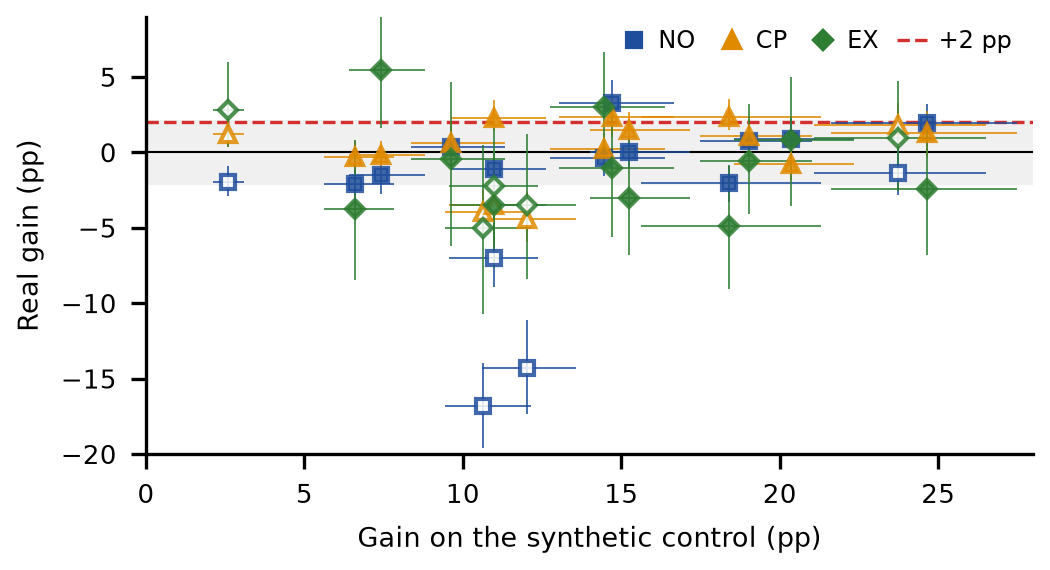
\includegraphics[width=\columnwidth]{fig_dispersion.png}
\caption{Gain on the synthetic control versus gain on each real source, with 95\,\% image-level CIs (17 blocks; filled: equal exposure; hollow: unequal or early; H3, with +60.9 on the control, is off scale). Grey band: $\pm2$ pp. Spearman $\rho$ with block-bootstrap CI over the 17 blocks: NO +0.37 [$-$0.11; +0.75], CP +0.24 [$-$0.21; +0.62], EX $-0.05$ [$-$0.55; +0.51]; with equal exposure (11), NO +0.63 [0.00; +1.00].}
\label{fig:disp}
\end{figure}

\textbf{Association and realism (post hoc analyses).} The association between each block's synthetic gain, measured on its own control, and the real gain is inconclusive: with equal exposure, on NightOwls $\rho=+0.63$ [0.00; +1.00] (Fig.~\ref{fig:disp}). With a control of coverage 0.35--0.70, like \emph{heavy}, all 15 blocks trained on ExDark pass (+2.1 to +33.6), and the association with the real gains is not positive either ($\rho$ from $-0.11$ to $-0.01$, $n=15$). For realism (H13, partially confirmed), a linear classifier on DINOv2~\cite{Oquab2024dinov2} tells truly occluded CityPersons people from those occluded by each family (AUC 0.935--0.993, $n=400$) better than from the same people unoccluded (0.876), and CLIP~\cite{Radford2021clip} agrees; on the occluded region, the KID distance~\cite{Binkowski2018kid} (unscaled) brings no family close to the real occluder. Training on CityPersons takes its \emph{heavy} to 0.59, against at most 0.24 without training there (a descriptive, uncontrolled comparison).

\textbf{Mechanism (exploratory).} With augmentation, recall on occluded NightOwls pedestrians drops in every block with a diagnosis, and with silhouettes and diffusion false positives also drop: the models miss occluded people with more confidence, a silent failure for surveillance.

\section{Discussion}
The results agree with Taori et al.~\cite{Taori2020shifts} and Pytel et al.~\cite{Pytel2021tilting}: what is gained against a synthetic perturbation barely carries over to the real one. They do not contradict Kassaw et al.~\cite{Kassaw2026occl}: synthetic occlusion can rank models and still not suffice as a training signal. As in Hendrycks et al.~\cite{Hendrycks2021manyfaces} and Mintun et al.~\cite{Mintun2021interaction}, carry-over depends on the augmentation--test pair: the only block that meets the rule (Faster R-CNN with silhouettes) is not repeated with other occluders or with RetinaNet, and its gain is fragile across seeds, is not occlusion-specific and, on CityPersons, consists partly of extending the box of partially visible people, something a region-based head could learn~\cite{Wang2017afast}. That passing the control is not enough is compatible with a shortcut~\cite{Geirhos2020shortcut}: the artificial occluder remains distinguishable from the real one (H13), although this has not been tested confirmatorily. We do not refute compositional architectures~\cite{Kortylewski2020compnet,Wang2020compnet}, amodal supervision~\cite{Reddy2022walt} or domain adaptation~\cite{Yi2022yolox}.

\textbf{Limitations.} \emph{Architecture:} six detectors and a single two-stage detector, with one backbone; RetinaNet uses another learning rate and loss, and the H16 V1 come from another machine. \emph{Data:} almost all real occlusion is in datasets other than the training one; CityPersons is daytime, NightOwls is recorded from a vehicle and the ExDark proxy captures only occlusion between people; evaluation is at 640 px; everything is AP@0.5 of one class. \emph{Protocol:} three seeds (five in the extension), with a hierarchical CI that underestimates them; 51 cells without multiplicity correction that share baselines; unequal exposure in the first blocks; the fingerprint has no third-party timestamp, and realism was measured in feature spaces.

\textbf{Future work.} (1) Occlusion mined from real images and amodal supervision~\cite{Reddy2022walt}. (2) Domain adaptation for night~\cite{Yi2022yolox} and part-based architectures~\cite{Wang2020compnet}. (3) Real night surveillance video annotated by visibility, with tracking: ByteTrack~\cite{Zhang2022bytetrack} and BoT-SORT~\cite{Aharon2022botsort} keep identities through brief occlusion by recovering low-confidence boxes, but only if the detector emits them. (4) Repeating H15--H17 with more seeds, V1 and V3 on the same machine and a matched recipe. For practice: a synthetic control is useful to check that an augmentation was learned, but claiming robustness requires annotated real occlusion from the deployment domain and a specificity measurement.

\section{Conclusion}
In 18 blocks with five kinds of occluder, six detectors and three training domains, synthetic occlusion augmentation always improved detection on synthetic occlusion. On real occlusion, with equal exposure, the mean gain was +1 pp on CityPersons, null on NightOwls and inconclusive on ExDark, and the only combination that met the rule, Faster R-CNN with silhouettes, did not withstand between-seed variance, specificity or the visible box. In person detection with pixel-level augmentation and fine-tuning from COCO, passing a synthetic control is not enough to claim robustness to real occlusion: it takes annotated real occlusion, V1 and V3 on the same machine and a specificity criterion.

\section*{Declarations}
\textbf{Data and code.} Code, logs, fingerprints, sampling lists and the supplement at \url{https://github.com/jhanrq8888/argos-occlusion-transfer} (public); trained weights will be deposited with a DOI on Zenodo upon publication. \textbf{Funding:} none. \textbf{Competing interests:} none. \textbf{Contributions (CRediT):} J.~L. Ramos Quispe: conceptualization, methodology, software, formal analysis, investigation, data curation and writing of the original draft; C.~P. Apaza Hilasaca: conceptualization, methodology (design of the pre-specification), review and editing; B.~R. Condori Quispe: data curation, validation, visualization, review and editing. \textbf{Use of AI:} the authors used Scopus AI (Elsevier) to support the search for seed articles, and Claude (Anthropic) for the search, the analysis code and drafting and editing the text. They reviewed and verified the code, results, references and text, for which they take full responsibility.

\bibliographystyle{IEEEtran}
\bibliography{references}

\end{document}
